% !TEX TS-program = pdflatexmk
\documentclass[12pt]{article}
\usepackage{float}

\usepackage{amsthm}

% Layout.
\usepackage[top=.75in, bottom=0.75in, left=.75in, right=.75in, headheight=1in, headsep=6pt]{geometry}

\usepackage{fancyhdr, enumerate,multirow}
% Fonts.
\usepackage{mathptmx}
\usepackage[scaled=0.86]{helvet}
\renewcommand{\emph}[1]{\textsf{\textbf{#1}}}

% Misc packages.
\usepackage{amsmath,amssymb,latexsym}
\usepackage{graphicx,tikz}
\usepackage{array}
\usepackage{xcolor}
\usepackage{multicol}
\usepackage{tabularx,colortbl}
\usepackage[T1]{fontenc}
\usepackage{enumitem}
%to make tikz pics work
\usepackage{tikz,pgfplots}

\usepackage{varwidth}
\usepackage{verbatim}

\newenvironment{centerverbatim}{%
  \par
  \centering
  \varwidth{\linewidth}%
  \verbatim
}{%
  \endverbatim
  \endvarwidth
  \par
}

\makeatletter
\newenvironment{centeredverbatim}{\expandafter\verbatim\centering}{\endverbatim}
\makeatother


\usetikzlibrary{arrows}
\newcommand{\midarrow}{\tikz \draw[-triangle 90] (0,0) -- +(.1,0);}

\usepackage[colorlinks=true]{hyperref}

% Paragraph spacing
\parindent 0pt
\parskip 6pt plus 1pt
\def\tableindent{\hskip 0.5 in}
\def\ts{\hskip 1.5 em}

\usepackage{fancyhdr}
\pagestyle{fancy} 
\lhead{\large\sf\textbf{MATH 663 }}
\rhead{\large\sf\textbf{Fall 2023}}
\chead{\large\sf\textbf{HW 4}}

\newcommand{\localhead}[1]{\par\smallskip\textbf{#1}\nobreak\\}%
\def\heading#1{\localhead{\large\emph{#1}}}
\def\subheading#1{\localhead{\emph{#1}}}

%% Special Math Symbol shortcuts
\newcommand{\NN}{\mathbb{N}}
\newcommand{\rad}{\text{rad}}
\newcommand{\diam}{\text{diam}}
\newcommand\solution{\localhead{Solution:}}

%\newenvironment{clist}%
%{\bgroup\parskip 0pt\begin{list}{$\bullet$}{\partopsep 4pt\topsep 0pt\itemsep -2pt}}%
%{\end{list}\egroup}%

\usetikzlibrary{calc,arrows.meta}
%\pgfplotsset{my style/.append style={axis x line=middle, axis y line=
%middle, xlabel={$x$}, ylabel={$y$}, axis equal }}


\begin{document}
\begin{enumerate}
	\item 
	\begin{enumerate}
		\item Find a bipartite graph with a set of preferences such that no matching of maximum size is stable and no stable matching has maximum size. 
		\solution Consider the following bipartite graph and preferences,
		
		
		\begin{figure}[H]
			\begin{center}
				\caption{Bipartite Graph, $G$}
				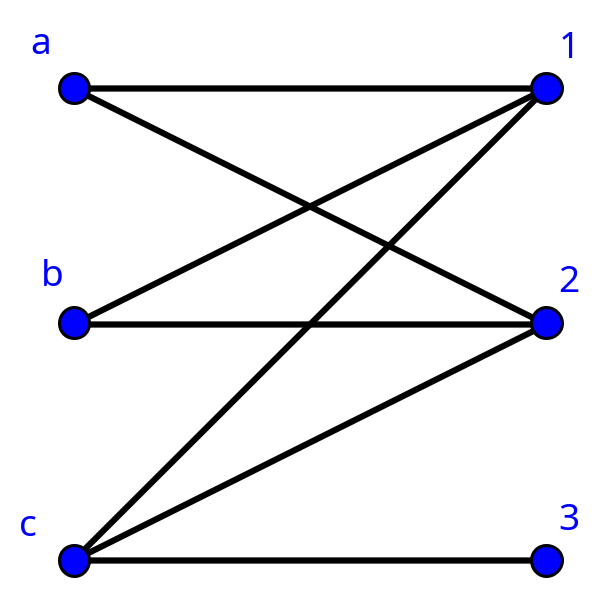
\includegraphics[width=.20\textwidth]{PartiteGraph.png}
			\end{center}
		\end{figure}
		\begin{table}[H]
			\caption{Preferences for $G$}
			\begin{center}
				\begin{tabular}{cccccccc cccccc}
					a:&2&>&1& & & \qquad\qquad    &1:&c&>&b&>&a\\ 
					b:&1&>&2& & & \qquad\qquad     &2:&c&>&a&>&b\\
					c:&1&>&2&>&3& \qquad\qquad &3:&c\\
				\end{tabular}
			\end{center}
		\end{table}
		Suppose $M$ is a matching of maximum size. Note $m$ must contain the edge $c3$ yet any matching that contains this edge must be unstable, since $c$ prefers vertices $1$ and $2$ over $3$ and vertices $1$ and $2$ prefer $c$ over $a$ and $b$. Therefore no matching of maximum size is stable. Let $M$ be a stable matching, note that $c$ will always be saturated by this matching by edge $c1$ and hence $M$ does not contain $c3$ and is therefore not a maximum matching
		
		
		
		
		
		
		
		
		\item Find a non-bipartite graph with a set of preferences that has no stable matching.
		\begin{proof}
			Consider a love triangle. 
		\end{proof}
	\end{enumerate}
	P.S: Just want to preface that this is not my best work, and very rushed, very sorry. 
	\newpage
	
	
	


\item Give an infinite family of examples that demonstrates that the \emph{bridgeless} hypothesis in Corollary 2.2.2 is necessary.
\begin{proof} Let $n \in \NN$ be an odd, such that $n > 3$. Now consider the rooted tree on $n$ vertices where every parent vertex, has two child vertices, unless they are leaves. Now connect the leaves by a cycle. Call this graph, $S_n$. Note that except for the root which has degree 2, this graph is 3-regular, and has odd degree. Now we construct a family of graphs which demonstrate the \emph{bridgeless} hypothesis in Corollary 2.2.2 is necessary. Let $G_n$ be a vertex $c$, adjacent to the root vertices of 3 $S_n$ graphs. Again note that now $G_n$ is 3-regular, $c$ has degree 3 and the degree of the root vertices in each $S_n$ component has been increased by 1 and are now 3. This graph also has 3 bridges incident to $c$. Applying Tutte's Theorem with $S = \{c\}$ we find that $q(G_n - S) = 3 \not \leq 1 = |S|$ and hence $G_n$ cannot have a 1-factor.  
\end{proof}
\newpage












\item A graph $G$ is called \emph{critically 2-connected} if $G$ is 2-connected but for every edge $e \in E,$ $G-e$ is no longer 2-connected.
	\begin{enumerate}
	\item Find an infinite family of critically 2-connected graphs that are not cycles.
	\begin{proof} Consider a cycle $C_n$ where $n \geq 4$, choose two antipodal vertices $u, v$ and form a path between them through a new vertex $c$. Call this new graph $C^*_n$, and note that this graph is clearly 2-connected, as you could remove any single vertex and remain connected. Note that $C^*_n$ is critically two connected, since of one were to remove any edge on the original cycle or on the new path the graph could be easily disconnected by removing either $u$ or $v$.


% any edge removed, removes a degree from a vertex that was originally degree 2




	\end{proof}
	\item Prove that if $G$ is 2-connected, then the statements below are equivalent:
		\begin{itemize}
		\item $G$ is critically 2-connected.
		\begin{proof} Let $G$ be two connected and suppose that $G$ is critically 2-connected. Suppose for the sake of contradiction that there exists an cycle $C$, in $G$ with a chord, call it $uv$. Note that in the cycle $C$ which is 2-connected, $C - uv$ remains 2-connected, since $C - uv$ is still a cycle. Thus $G - uv$ is 2-connected. 
			
		\end{proof}



		\item No cycle in $G$ has a chord.
		\begin{proof} Let $G$ be 2-connected and suppose that no cycle in $G$ has a chord. Suppose for the sake of contradiction that $G$ is not critically 2-connected. Therefore there exists an edge $e$ such that $G - e$ is still 2-connected. Let $x, y \in G$ incident to $e$. Since $G - e$ is 2 connected, $G - e$ is at least 2-edge connected. By Menger's Theroem there exists at least 2 edge-disjoint paths between $a$ and $b$ in $G - e$. These paths form a cycle, and hence $e$ was a chord in a cycle in $G$ a contradiction.   
		\end{proof}
		\end{itemize}
	\end{enumerate}
\newpage









\item Prove that the block graph of any connected graph is a tree.
\begin{proof} Suppose $G$ is a connected graph, and let $\mathcal{B}(G)$ be it's block graph. 
	Let $u, v \in \mathcal{B}(G)$ and note that $u$ and $v$ can represent a block or a cut vertex in $G$. Since each block in $G$ contains a cut vertex, every vertex in $\mathcal{B}(G)$ which represents a block in $G$, is adjacent to a vertex which represents a cut vertex in $G$ therefore to show that $\mathcal{B}(G)$ is connected, it is sufficient to show that there exists a path between any two vertices which represent a cut vertex in $G$. 
	Let $u$ and $v$ represent cut vertices such that $u \neq v$. Since $G$ is connected there exists a $uv$ path in $G$. In $\mathcal{B}$ this path is represented by a path for some $n \geq 1$ such that $uB_1a_1B_2,\dots, B_nv$, where $B_n$ are vertices which represent blocks and $a_n$ are cut vertices in $G$. 


	We wish to show that that $\mathcal{B}(G)$ is a cyclic. By construction $\mathcal{B}(G)$ is a bipartite graph, and therefore has no odd cycles. Suppose for the sake of contradiction that there exists an even cycle $C$, in $\mathcal{B}(G)$. Let without loss of generality let $C = a_1B_1a_2, ...B_na_1$, now note that this cycle can be lifted into $G$ by simply choosing a path $P_i \subseteq B_i$ which between $a_i$ and $a_{i + 1}$. Therefore there exists a cycle in $G$, $C_G$ such that $a_1P_1a_2...P_na_1$. Since this is a cycle, not contained in a single block we have contradicted that the cycle of $G$ are the cycles of its blocks.  


\end{proof}
\newpage 







\item Use Menger's Theorem to prove that the statements below are equivalent:
\begin{itemize}
	\item $G$ is 2-connected.
	\item Every pair of vertices of $G$ lie on a common cycle.
	\item Every pair of edges of $G$ lie on a common cycle, $G$ is connected
\end{itemize}


\begin{proof}$(a \rightarrow b)$ Suppose $G$ is 2-connected and let $u, v \in V(G)$, by (global) Menger's Theorem, $G$ contains 2 independent paths between $u$ and $v$, call them $P_1$ and $P_2$. Note that $P_1$ and $P_2$ form a common cycle in $G$.\\
\end{proof}


\begin{proof}
$(b \rightarrow a)$ Suppose every pair of vertices of $G$ lie on a common cycle.
	Let $u, v \in V(G)$ such that both vertices lie on $C$, a common cycle in $G$. Then there exists two vertex disjoint paths $P_1$ and $P_2$. By (global) Menger's Theorem $G$ is 2-connected. 
\end{proof}

\begin{proof}$(a \rightarrow c)$. Suppose $G$ is 2-connected, and consider edges $u_0v_0$ and $u_1v_1$ in $G$. Add the following $H$-paths $u_0av_0$ and $u_1bv_1$ to the graph and call it $G'$. Note since we added $H$-paths to a 2-connected graph $G'$ is still 2-connected. Now we apply Menger's Theorem to $G'$, choosing disconnecting sets $\{a\}$ and $\{b\}$. Again since $G'$ is two connected the minimum number ov vertices separating $a$ and $b$ is 2, and therefore by Menger's Theorem the maximum number of disjoint $a-b$ paths in $G'$ is 2, call them $P_1$ and $P_2$. Since $a$ and $b$ only have two neighbors, these disjoint $a-b$ paths must contain the following, without loss of generality $v_0, v_1 \in P_1$ and $u_0, u_1 \in P_2$. It follows that, in $G$, edges $u_0v_0$ and $u_1v_1$ form a cycle with $P_1 - \{a, b\}$ and $P_2 - \{a, b\}$. Hence any two edges lie on a cycle in $G$. 
\end{proof}


\begin{proof}$(c \rightarrow b)$ Suppose $G$ is connected an any two edges lie on a common cycle. Let $a, b \in G$, and note that  since $G$ is connected we can let $e_1$ be incident to $a$ and $e_2$ be incident to $b$ such that $e_1 \neq e_2$. Let $C$ be the common cycle containing both $e_1$ and $e_2$. This cycle must contain $a$ and $b$
\end{proof}
\newpage






\item Given a graph $G=(V,E),$ the \emph{line graph of $G$}, denoted $L(G)$ has vertex set $E$ and two vertices $e,f \in E$ are adjacent in $L(G)$ if and only if $e$ and $f$ are incident in $G$.	



\begin{enumerate}
	\item Determine $L(G)$ for $P^m,$ $C^k$ and $H$ (graphed below).\\
	
	%%%BEGIN Graph G
	\begin{center}
		
		\begin{tikzpicture}[scale=1,every node/.style={draw,circle, inner sep=.05 cm}]
			\foreach \i in {0,1,2,3,4}{
				\node (\i) at (\i*72+18:2){};
				}
				\node (5) at (27:3){};
				\node (6) at (9:3){};
				\draw (6)--(0)--(1)--(2)--(3)--(4)--(0)--(5);
			\end{tikzpicture}
		\end{center}
		
		
		
		\begin{proof} Note that in the $L(P^m)$ the interior vertices of $P^m$ get mapped to edges and the edges get mapped to vertices. Hence $L(P^m) = P^{m - 1}$. A similar argument gets us that $L(C^k) = C^{k}$, since there are $k$ edges in a $C^k$. Below is $L(H)$ denoted by the red edges and black square vertices,
			\begin{figure}[H]
				\begin{center}
					\caption{$L(H)$ in red, and $H$ in blue.}
					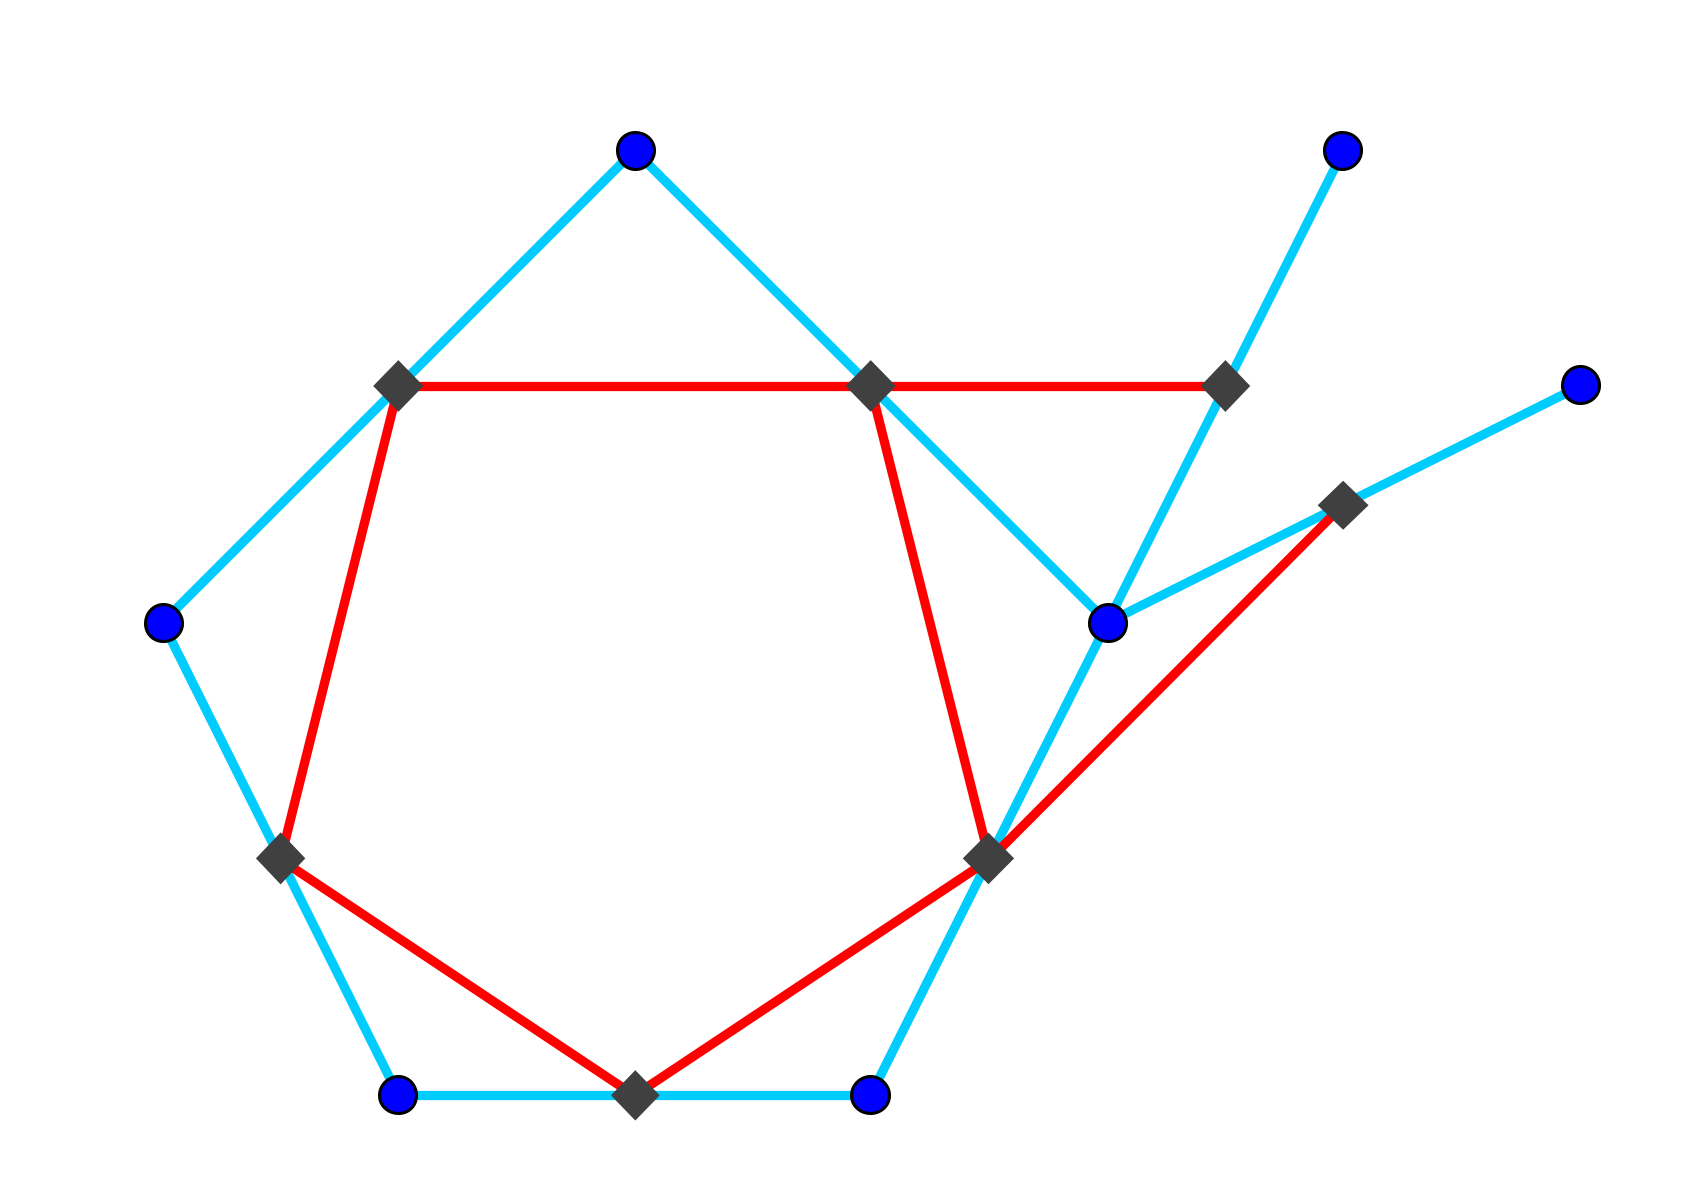
\includegraphics[width=.50\textwidth]{LineGraph.png}
				\end{center}
			\end{figure}




		\end{proof}




		\item Show that a cut set of vertices in $L(G)$ must correspond to a cut set of edges of $G$, but that the reverse does not necessarily hold.
		\begin{proof} Let $G$ be a connected graph and let $S$ be a cut set of vertices in $L(G)$ suppose for the sake of contradiction that $S$ corresponds to a set of edges $E$, that does not disconnect $G$. Note that by definition $L(G - E) = L(G) - S$ however $G - E$ is connected and $L(G) - S$ is disconnected, a contradiction. 
		\end{proof}

		\begin{proof} As a counter example to show that the reverse does not hold, consider 
			a $C_5$ and note that $L(C_5) = C_5$. Choose a cut set of edges to be a pair of edges $e_1$ and $e_2$ which are incident to the same vertex in $C_5$. Note that in $L(C_5)$, $e_1$  and $e_2$ correspond to two adjacent vertices a cycle, which once removed the graph remains connected. 
		\end{proof}














		\end{enumerate}
%%%END Graph G
	
\end{enumerate}
\end{document}


